\documentclass{standalone}
\usepackage{tikz} % tikz
\usepackage{standalone} % tikz figures are often in standalone
\usepackage{amsfonts} % mathbb etc
\usepackage{amsmath} % crucial package
\usepackage{amsthm} % ams-style theorems
\usepackage{bm} % bold math symbols
\usepackage{xcolor} % more colors
\usepackage[T1]{fontenc} % modern encoding, better than OT1, the default

\newtheorem{definition-fr}{Définition}
\newtheorem{example-fr}{Exemple}
\newtheorem{theorem-fr}{Théorème}
\newtheorem{proposition-fr}{Proposition}
\newtheorem{lemma-fr}{Lemme}
\newtheorem{remark-fr}{Remarque}
\newtheorem{definition}{Definition}
\newtheorem{lemma}{Lemma}
\newtheorem{proposition}{Proposition}
\newtheorem{remark}{Remark}

\usetikzlibrary{decorations.pathmorphing} % for snake, zigzag...
\usetikzlibrary{positioning} % for the "below of=1cm" type of options
\usetikzlibrary{intersections} % e.g. for pyramid
\usetikzlibrary{calc} % for computing node coordinates from others
\usetikzlibrary{overlay-beamer-styles} % when \pause glitches in tikz beamer
\usetikzlibrary{arrows} % arrows
\usetikzlibrary{external} % only compile the figure the first time
\tikzexternalize[only named=true, prefix=tikz-cache/]
\immediate\write18{mkdir -p latex-build/tikz-cache}

% used to pass "scale=XX" as includetikz option
\pgfkeys{
  /tikzoptions/.is family, % Namespace
  /tikzoptions/.cd, % Namespace
  scale/.store in=\scale, % Store the value of 'scale'
}

% usage: \includetikz[scale=XX]{fig}, fetches from my local database
\newcommand{\includetikz}[2][scale=1]{
  \bgroup
  \pgfkeys{/tikzoptions,#1} % currently only accepts 'scale' (april 9 2025)
  \tikzsetnextfilename{#2}
  \include{tex-macros/tikz-figures/#2}% Include the standalone TikZ file
  \egroup
}

% usage: \inputtikz[scale=XX]{fig}, fetches from my local database
\newcommand{\inputtikz}[2][scale=1]{
  \bgroup
  \pgfkeys{/tikzoptions,#1} % currently only accepts 'scale' (april 9 2025)
  \tikzsetnextfilename{#2}
  \input{tex-macros/tikz-figures/#2}% Include the standalone TikZ file
  \egroup
}


\newcommand{\bigOt}{\widetilde{\mathcal{O}}}
\newcommand{\bigO}{\mathcal{O}}

\definecolor{mypurp}{HTML}{8f0c97}
\definecolor{myred}{HTML}{9f103b}
\definecolor{myor}{HTML}{ae3011}
\definecolor{mydarkor1}{HTML}{96240f}
\definecolor{mydarkor2}{HTML}{7f180c}
\definecolor{mylb1}{HTML}{00557e}
\definecolor{mylb2}{HTML}{013157}
\definecolor{mybl1}{HTML}{0d08a9}
\definecolor{mybl2}{HTML}{04037f}
\definecolor{mygr1}{HTML}{097e3e}
\definecolor{mygr2}{HTML}{025520}
\definecolor{myyellow}{HTML}{FFD700}



\makeatletter
\@ifundefined{scale}{
  \def\scale{1}
}
\makeatother


\begin{document}
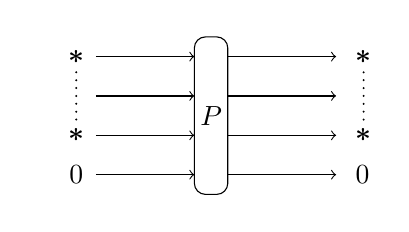
\begin{tikzpicture}[scale=\scale]
    \def\arrowlength{1.5cm}
    \def\branchdistance{.5cm}

    \foreach \z in {1,...,4} {
      \node[] (x\z) at ($\z*(0,-\branchdistance)$)  {};
      \node[] (y\z) at ($(\arrowlength,-\z*\branchdistance)$) {};
      \draw[->] (x\z) -- (y\z);
    }

    \node[] (star1) at (x1.west) {$\bm{*}$};
    \node[] (star2) at (x3.west) {$\bm{*}$};
    \draw[dash pattern=on 0pt off 1mm, line cap=round, thick] ($ (star1) + (0,-0.4*\branchdistance) $) -- ($ (star2) - (0,-0.4*\branchdistance) $);
    \node[] at (x4.west) {$0$};

    \node[] (r1) [left=0.5cm of x1.north] {};
    \node[] (r2) [left=0.5cm of x3.south] {};

    \draw (y1.west) +(0,.5*\branchdistance) node (rect1) {};
    \draw (y4) +(.3cm,-.5*\branchdistance) node (rect2) {};

    \draw[rounded corners] (rect1) rectangle (rect2) node[pos=0.5] {$P$};

    \foreach \z in {1,...,4} {
      \node[] (xx\z) at (rect2.west |- y\z)  {};
      \draw[->] (xx\z) -- +(\arrowlength,0) node (yy\z) {};
    }

    \def\outputoff{0mm}
    \node[] (star3) [right=\outputoff of yy1] {$\bm{*}$};
    \node[] (star4) [right=\outputoff of yy3] {$\bm{*}$};
    \draw[dash pattern=on 0pt off 1mm, line cap=round, thick] ($ (star3) + (0,-0.4*\branchdistance) $) -- ($ (star4) - (0,-0.4*\branchdistance) $);
    \node[] (yyy4) [right=\outputoff of yy4] {$0$};
  \end{tikzpicture}
\end{document}


